% ============================================================
%  Desk trebuchet -- clip-together kit: cutting + assembly guide
%  Drawings from steps_desk.py; files from gen_desk.py
% ============================================================
\documentclass[11pt,a4paper]{article}
\usepackage[T1]{fontenc}
\usepackage[a4paper, top=1.2cm, bottom=1.6cm, left=1.5cm, right=1.5cm]{geometry}
\usepackage{xcolor}
\usepackage{graphicx}
\usepackage{booktabs}
\usepackage{array}
\usepackage{tabularx}
\usepackage{enumitem}
\usepackage{fancyhdr}
\usepackage{amssymb}
\usepackage[protrusion=true,expansion=false]{microtype}

\definecolor{Ink}{HTML}{1A1A1A}
\definecolor{HeadGrey}{HTML}{333333}
\definecolor{RuleGrey}{HTML}{888888}
\definecolor{LineGrey}{HTML}{555555}
\definecolor{WarnBg}{HTML}{F5F5F5}
\definecolor{Badge}{HTML}{C0392B}
\definecolor{NeedBg}{HTML}{F6F1E7}
\definecolor{CutRed}{HTML}{FF0000}
\definecolor{EngBlue}{HTML}{0000FF}

\setlength{\parindent}{0pt}
\setlength{\parskip}{3pt}
\renewcommand{\arraystretch}{1.15}
\newcolumntype{L}[1]{>{\raggedright\arraybackslash}p{#1}}
\newcolumntype{Y}{>{\raggedright\arraybackslash}X}

\newcommand{\parthead}[2]{%
  \par\vspace{2pt}\noindent
  \colorbox{HeadGrey}{\parbox{\dimexpr\linewidth-2\fboxsep}{\color{white}\large\bfseries #1\hfill\normalsize\mdseries #2}}\par\vspace{4pt}}
\newcommand{\sechead}[1]{%
  \par\vspace{5pt}{\bfseries\large\color{HeadGrey} #1}\\[-4pt]
  {\color{RuleGrey}\rule{\linewidth}{0.8pt}}\par\vspace{1pt}}
\newcommand{\badge}[1]{\colorbox{Badge}{\color{white}\bfseries\large\,#1\,}}
\newcommand{\need}[1]{\par\vspace{3pt}\noindent\colorbox{NeedBg}{\parbox{\dimexpr\linewidth-2\fboxsep}{\footnotesize\textbf{You need:} #1}}\par}
\newcommand{\warn}[1]{\par\vspace{3pt}\noindent\fcolorbox{LineGrey}{WarnBg}{\parbox{\dimexpr\linewidth-2\fboxsep-2\fboxrule}{\footnotesize #1}}\par}
\newcommand{\step}[5]{%
  \par\vspace{6pt}\noindent
  \begin{minipage}[t]{#4\linewidth}\vspace{0pt}\centering\includegraphics[width=\linewidth]{#3}\end{minipage}\hfill
  \begin{minipage}[t]{\dimexpr0.97\linewidth-#4\linewidth\relax}\vspace{0pt}
    \badge{#1}\;{\bfseries\large #2}\par\vspace{4pt}\small #5
  \end{minipage}\par\vspace{4pt}{\color{RuleGrey!50}\rule{\linewidth}{0.4pt}}}

\pagestyle{fancy}
\fancyhf{}
\renewcommand{\headrulewidth}{0pt}
\fancyfoot[L]{\footnotesize\color{RuleGrey} Desk trebuchet \textbullet{} clip-together kit}
\fancyfoot[R]{\footnotesize\color{RuleGrey} Page \thepage}

\begin{document}
\small

{\LARGE\bfseries\color{Ink} Desk trebuchet --- clip-together kit}\\[2pt]
{\large One sheet of 6\,mm plywood \textbullet{} no glue \textbullet{} slotted masses in a weight basket}\\[2pt]
{\color{RuleGrey}\rule{\linewidth}{1.2pt}}

A desk-sized trebuchet (400\,mm throwing arm) cut from \textbf{one 900 $\times$ 600 sheet of 6\,mm plywood} (every part sits inside the middle 850 $\times$ 550, leaving 25\,mm clear at each edge), that students clip together in about \textbf{10 minutes} and take apart flat again. There is \textbf{no glue}: the parts lock with hooked tabs, lock plugs, tapered keys and dovetails, and two bolts with wing nuts. The counterweight is a \textbf{plywood basket} that hangs from the arm and holds the school's slotted masses, so changing the counterweight takes seconds --- the variable changed in the investigation.

\begin{minipage}[t]{0.53\linewidth}
\sechead{Expected range (25\,g sand-filled beanbag)}
{\footnotesize
\begin{tabularx}{\linewidth}{@{}Y c c c c@{}}
\toprule
\textbf{Masses in the basket} & 400\,g & 600\,g & 800\,g & 1000\,g \\
\midrule
Plan on & 2\,m & 3.5\,m & 5\,m & 7\,m \\
Best case & 3\,m & 5\,m & 7.5\,m & 10\,m \\
\bottomrule
\end{tabularx}}

{\footnotesize From the computer model (the empty basket adds about 120\,g). ``Plan on'' is 30\,\% less for real-world losses. Peak arm spin about 11--16\,rad/s. A corridor, hall or the oval.}
\end{minipage}\hfill
\begin{minipage}[t]{0.44\linewidth}
\sechead{Not laser-cut}
{\footnotesize
\begin{tabularx}{\linewidth}{@{}Y r@{}}
\toprule
M8$\times$150 bolt, 2 washers, wing nut (axle) & 1 \\
M6$\times$100 bolt, 2 washers, wing nut (hang pin) & 1 \\
Thin strong cord (sling, trigger loop, pull cord) & 2\,m \\
100\,g slotted masses & up to 10 \\
25\,g sand-filled beanbags & 2+ \\
Rubber bands or hook-and-loop strap (sensor) & 2 \\
\bottomrule
\end{tabularx}}
\end{minipage}

\sechead{Cutting}
\begin{minipage}[t]{0.52\linewidth}\vspace{0pt}
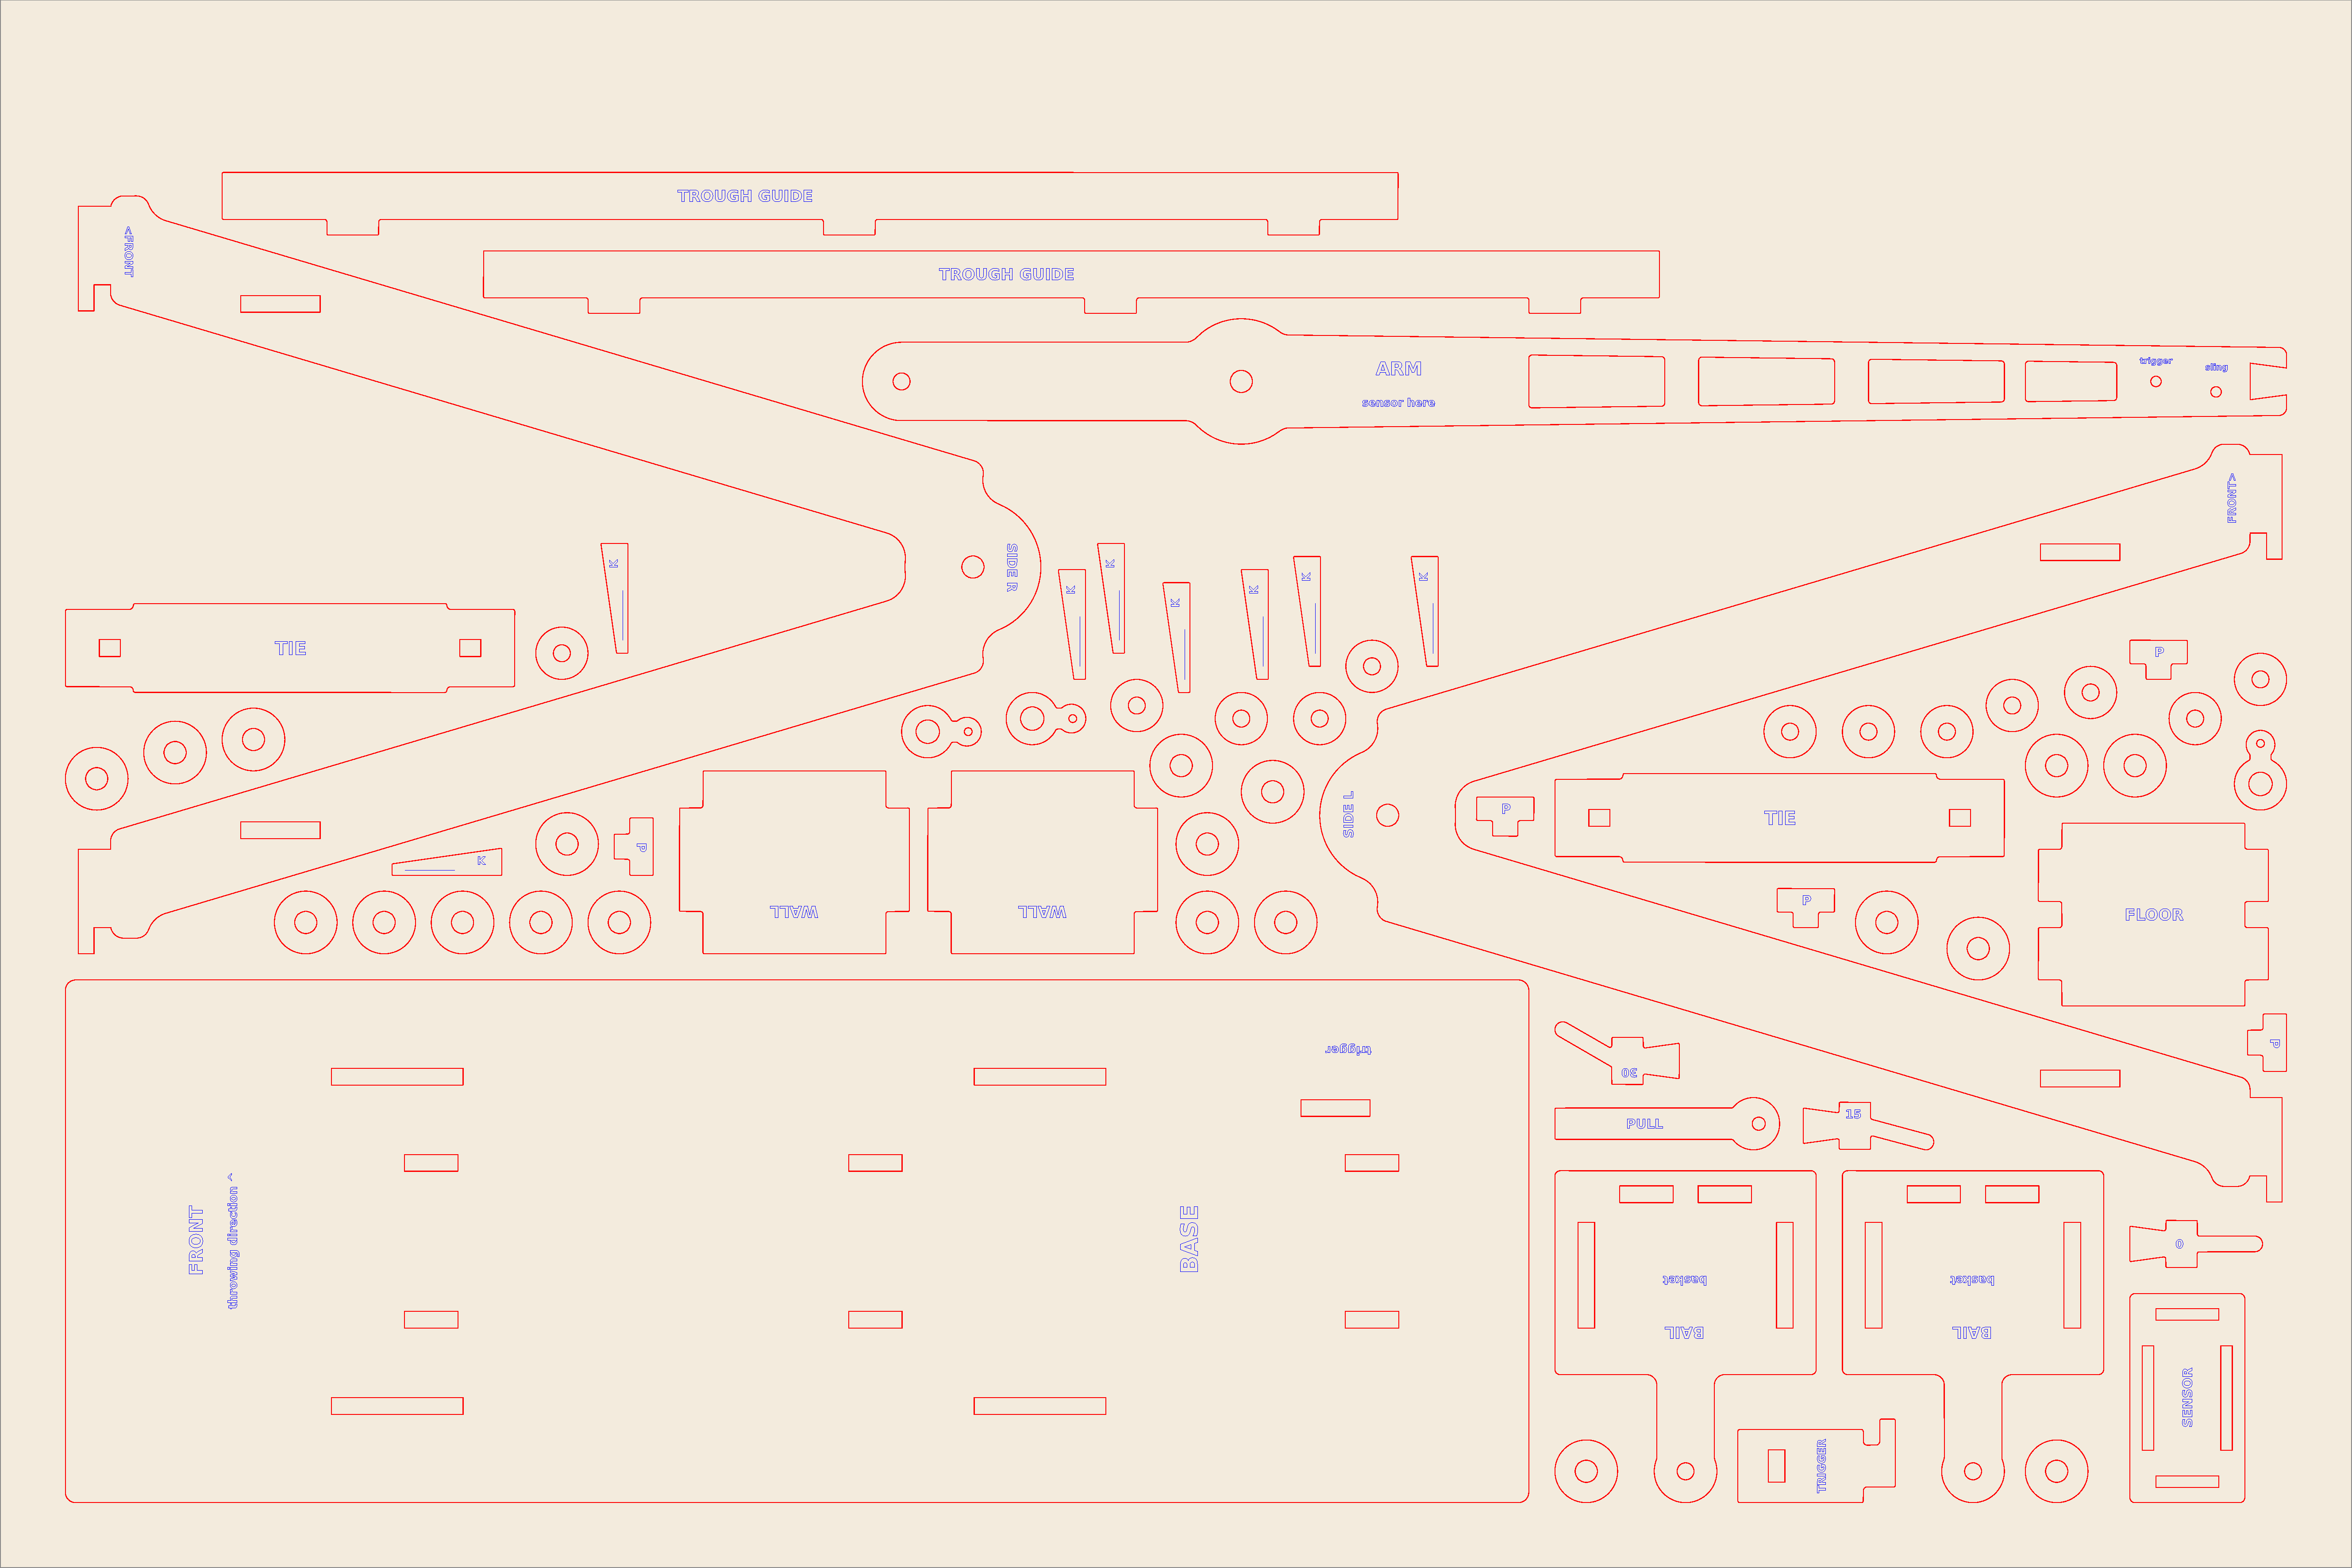
\includegraphics[width=\linewidth]{out/01_Desk_trebuchet_sheet1_preview.pdf}
\end{minipage}\hfill
\begin{minipage}[t]{0.45\linewidth}\vspace{0pt}
\begin{itemize}[itemsep=1pt, leftmargin=1.1em, topsep=0pt]
  \item \textbf{01\_Desk\_trebuchet\_sheet1} (.dxf / .svg): the whole kit on one sheet --- 67 parts including spares.
  \item \textbf{00\_Test\_coupon\_cut\_first}: cut this first. Find the slot a 6\,mm part pushes into firmly by hand, and check the 8 and 6\,mm bolts pass through their holes. There are two sets of files: \texttt{out} (slots drawn 6.4\,mm, about 6.6 after cutting) and \texttt{out\_CL0} (slots drawn 6.0\,mm, about 6.2 after cutting). Use the set whose middle coupon slot fits best. For another width, run \texttt{python3 gen\_desk.py --cl 0.2} (the number is mm over 6).
  \item \textbf{02\_Fabric\_pouches}: sling pouches in felt or canvas.
  \item \textcolor{CutRed}{\textbf{Red}} = cut; \textcolor{EngBlue}{\textbf{blue}} = engrave (labels). Engrave first.
  \item \textbf{Spares on the sheet:} 1 lock plug, 4 tie keys, 2 axle and 2 hang washers, 2 sling rings. The three release tips (0, 15, 30\textdegree) are for tuning.
\end{itemize}
\end{minipage}

\clearpage
\parthead{Assembly}{two students \textbullet{} about 10 minutes \textbullet{} no glue, no tools}

\step{1}{Check the parts}{steps/d01_inventory.pdf}{0.55}{%
Count the parts against the drawing. The two sides are mirror images: \textbf{SIDE L} and \textbf{SIDE R} are engraved on them.
\need{everything on the sheet, plus the bolts and cord.}}

\step{2}{Trough guides into the base}{steps/d02_guides.pdf}{0.52}{%
Lay the base engraved side up, ``FRONT'' pointing the way you will throw. Press each trough guide's three tabs into the slots down the middle of the base. They are a firm push fit.}

\step{3}{Clip in the sides}{steps/d03_sides.pdf}{0.52}{%
\begin{enumerate}[itemsep=0pt, leftmargin=1.3em, topsep=2pt]
  \item Hold a side upright, engraving facing \textbf{out}, and drop its two foot hooks through the long slots near the edge of the base.
  \item Slide the side \textbf{10\,mm back}: the hooks catch under the base.
  \item Push a \textbf{lock plug} into the gap that opens at the front of each slot. The side can't slide or lift out now.
\end{enumerate}
Do the same for the other side.
\need{2 sides, 4 lock plugs.}}

\step{4}{Ties and keys}{steps/d04_ties.pdf}{0.52}{%
Push each tie through the matching slots in both sides' legs (front and back). Push a tapered \textbf{key} through the hole in each tie end, just outside the side, thin end first and lying \textbf{flat}, with its \textbf{straight edge} (the one with the engraved line) against the side. Push it in until it is firm. The frame is now rigid.
\need{2 ties, 4 keys.}}

\step{5}{Trigger}{steps/d05_trigger.pdf}{0.45}{%
Drop the trigger post's hook through the small slot beside the trough at the back, slide it \textbf{forward}, and push a lock plug in behind it. Slide the trigger key through the slot in the post, handle on the outside, and tie a 1\,m pull cord to its handle.
\need{trigger post, trigger key, 1 lock plug, pull cord.}}

\step{6}{Get the arm ready}{steps/d06_arm.pdf}{0.55}{%
\begin{enumerate}[itemsep=0pt, leftmargin=1.3em, topsep=2pt]
  \item Slide the \textbf{15\textdegree{} release tip} into the dovetail at the end of the arm, prong pointing to the side marked \emph{sling}.
  \item \textbf{Sling:} tie a 400\,mm cord through the \emph{sling} hole and through one end of a pouch; tie a sling ring to the other end of the pouch with a second cord, so the pouch's centre is 360\,mm from the tip.
  \item Tie a short loop of cord (about 120\,mm round) through the \emph{trigger} hole.
  \item Strap the sensor plate where it says \emph{sensor here}, and the sensor to it.
\end{enumerate}}

\step{7}{Hang the basket on the arm}{steps/d07_basket.pdf}{0.46}{%
\begin{enumerate}[itemsep=0pt, leftmargin=1.3em, topsep=2pt]
  \item Push the M6 bolt through: washer, \textbf{bail}, 5 small washers, the arm's hang hole, 5 small washers, the other bail, washer, wing nut.
  \item Drop the floor's tabs into the bottom slots of both bails, and each wall's tabs into the side slots.
  \item Tighten the wing nut until the bails just hold the floor and walls; the basket must still swing on the bolt.
\end{enumerate}
\need{2 bails, floor, 2 walls, M6 bolt + wing nut, 10 small washers.}}

\step{8}{Fit the arm}{steps/d08_axle.pdf}{0.48}{%
Hold the arm upright between the sides with the basket hanging below. Push the M8 bolt through: washer, side, \textbf{9 large washers}, the arm, 9 large washers, the other side, washer, wing nut. Tighten the wing nut until snug, then back it off slightly: the arm must swing freely.
\need{M8 bolt + wing nut, 18 large washers.}}

\clearpage
\parthead{Launching}{teacher supervises \textbullet{} safety glasses on}

\noindent\begin{minipage}[t]{0.55\linewidth}\vspace{0pt}\includegraphics[width=\linewidth]{steps/d09_cocked.pdf}\end{minipage}\hfill
\begin{minipage}[t]{0.43\linewidth}\vspace{0pt}\small
\begin{enumerate}[itemsep=2pt, leftmargin=1.4em, topsep=0pt]
  \item Put the slotted masses in the basket, with the arm hanging at rest.
  \item \textbf{Cock it:} pull the tip of the arm down to the back. Hook the trigger loop over the trigger key, between the post and the trough.
  \item \textbf{Load it:} lay the sling in the trough with a beanbag in the pouch, and drop the ring over the release tip.
  \item Everyone behind the trebuchet. The operator holds the pull cord from the side and calls \textbf{``Firing''}.
  \item Pull the cord: the key slides out and the loop lets go.
  \item Wait until the arm stops before anyone touches it.
\end{enumerate}
\end{minipage}

\sechead{Tuning}
{\footnotesize
\begin{tabularx}{\linewidth}{@{}L{5.8cm} Y@{}}
\toprule
\textbf{What you see} & \textbf{What to change} \\
\midrule
Beanbag goes straight up, or backwards & Releases too early: swap to the \textbf{0\textdegree{}} release tip. \\
Beanbag hits the ground just in front & Releases too late: swap to the \textbf{30\textdegree{}} tip. \\
Beanbag flies off to one side & Sling cords uneven, or the beanbag isn't in the middle of the trough. \\
Arm stiff or slows quickly & Back the axle wing nut off a little; check the washers aren't pinched. \\
Frame rocks & Check the four keys and the four lock plugs are pushed fully home. \\
\bottomrule
\end{tabularx}}

\warn{\textbf{Safety.} Safety glasses for everyone near it. Launch along an empty corridor or hall, away from windows, with nobody in front of the trebuchet or within 1\,m of its sides. Beanbags only. Change the masses only with the arm at rest. Keep fingers out of the frame while it is cocked: the basket swings down hard.}

\parthead{Pack down}{about 5 minutes}
Masses out first. Then reverse the assembly: arm off the axle bolt; basket off the arm (keep the washers on the bolts so they don't get lost); keys out, ties out; lock plugs out, slide each side forward and lift it out; guides out. Everything packs flat --- store each kit in its own A3 envelope or tray with its bolts, cord, washers and spares.

\end{document}
